\documentclass{llncs}
\usepackage{graphicx}
\usepackage[utf8]{inputenc}
\begin{document}

\title{Matching de Formes}

\author{Julien ALTIERI, Benoit SEGUIN, Frédéric WILHELM\institute{Ecole Polytechnique, X2008}}



\maketitle

\begin{abstract}
Le \textit{matching de formes} est un probl\`eme r\'ecurrent de g\'eom\'etrie algorithmique. Il s'agit d'une part d'\'evaluer la \textit{proximit\'e g\'eom\'etrique} de deux maillages ind\'ependamment de ces maillages, et d'autre part de trouver une \textit{transformation rigide} qui envoie l'un sur l'autre, de mani\`ere optimale. Le d\'efi consiste donc à extraire des propri\'et\'es g\'eom\'etriques \textit{intrins\`eques} de l'objet, ce que nous faisons en exploitant le \textit{tenseur de courbure}. \textbf{suite \`a expliquer pour la transformation rigide}.
\end{abstract}

\section{Introduction, motivation, ...}
Nous souhaitions au d\'epart d\'evelopper un jeu de sculpture, avec des formes \`a reproduire. Cet objectif nous a naturellement conduit \`a devoir \'evaluer un score de proximit\'e, et donc au matching de forme.


%si on veut faire une figure (ceci est un commentaire => retirer les % pour decommenter)
%\begin{figure}
%\center
%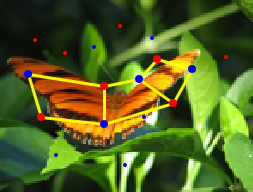
\includegraphics[bb=0 0 253 192, width=5cm]{relevantinformation.png}
%\caption{un commentaire ?}
%\end{figure}



\section{Organisation du code}

Nous choisissons d'implémenter deux versions différentes de la courbure, nous utilisons donc une classe abstraite \texttt{CourbureEstimator} qui comporte essentiellement une méthode \texttt{double compareTo(CourbureEstimator c)} renvoyant la distance entre les deux maillages, et une méthode \texttt{void computeSignature()} qui évalue la courbure suivant la méthode utilisée. Deux classes l'implémentent : \texttt{GaussianCourbureEstimator}

pour la méthode de Gauss, et \texttt{Taubin} pour le tenseur de courbure. Le programme principal se situe dans la classe \texttt{Matching}


\section{Courbure de Gauss}

La première manière et la plus simple de calculer la courbure en un point est la courbure de Gauss. En version discrète, elle s'exprime par la formule suivante :
 \[ \kappa_G(v) = \frac{3(\sum_{i}\theta_{i}-2\pi)}{\sum_{i}  Aire(F_{i})}  \]
Cette formule permet d'obtenir instantanément le produit des courbures principales. Ainsi, en effectuant un passage sur chacun des points on obtient une distribution de la courbure de Gauss du maillage. 

Comme l'on essaye de traiter le problème en étant indépendant par rapport à l'échelle, on impose une certaine moyenne à la distribution des courbures. On divise donc toutes les valeurs par la moyenne désirée, puis grâce à un $ arctan $ on peut transposer l'intervalle non borné des courbures dans un intervalle $ \left[ -1 ; 1 \right] $.


\section{Taubin}

\subsection{\'Evaluer le tenseur de courbure}

Une seconde méthode consiste à utiliser l'algorithme de Taubin ~\cite{taubin} pour évaluer un tenseur de courbure sur notre maillage. Ce tenseur représente l'application bilinéaire en un point du maillage, qui à un vecteur direction (dans le plan tangent à la surface) associe la valeur de la courbure suivant cette direction. C'est un donc tenseur 2x2 que l'on va diagonaliser.
\\\\
Sa base de diagonalisation est constituée des deux directions principales de courbure (orthogonales dans cette approximation). Les valeurs propres associÈes sont les courbures selon ces directions et servent à comparer deux maillages.

\subsection{Calcul de la signature}

Dans le cas d’estimation de courbure précédent (courbure de Gauss), à chaque point correspondait une unique courbure, donc un unique nombre. L’établissement d’une signature consistait donc à recenser les différentes courbures. Dans le cas présent, chaque point est caractérisé par deux valeurs propres du tenseur de courbure. Il s’agira donc d’effectuer un recensement en deux dimensions.
\\\\
On implémente donc la signature par une matrice de valeurs réelles à deux dimensions $S_{i,j}$, de taille donnée selon la résolution voulue, par exemple $ 512 \times 512 $. Pour chaque vertex $ v $ ayant comme courbures $ c1$ et $c2 $, on va incrémenter $ S_{i,j} $ où $i$ et $j$ sont fonction de v (on incrémente également $ S_{j,i} $ car les deux valeurs propres ne sont pas ordonnées). Chaque point ``vote'' donc pour un couple de courbure :
$$
S_{i,j} = S_{j,i} = \# \{v\in V|f(c_1(v))=i \mbox{ et } f(c_2(v))=j \}
$$
où $f$ est une fonction à définir.
\\\\
Pour déterminer $f$, il est nécessaire de s’intéresser aux problèmes d’échelle et d’échantillonnage : en effet, même si deux maillages que l’on souhaite comparer ont intuitivement et visuellement ``la même forme'', rien ne dit qu’ils ont la même échelle, ni le même échantillonnage (nombre de vertex). Pire encore, il se peut que pour deux formes similaires, les densités d’échantillonnage varient au sein de la même forme, et perturbent le vote.
\\\\
Pour l’échantillonnage, le problème se résout en pondérant les votes des points par leurs poids, où l’on définit le poids $w$ d’un sommet par la somme des surfaces des faces avoisinantes :
$$
\forall v\in V, w(v) = \sum_{i}{A(f_i)},
$$
Où les $f_i$ sont les faces voisines de v, et $A(f_i)$ leurs aires.
\\\\
Quand à l'indépendance vis-à-vis de l'échelle, nous avons choisi d’effectuer, pour chaque maillage, une homothétie sur l’ensemble des courbures de telle sorte que la moyenne soit la même. Ainsi, la carte des courbures n’est pas modifiée si on agrandit la forme.
%$$
%M = \frac{\sum_{v\in V}{w(v) \frac{c_1(v) + c_2(v)}{2}}}{\sum_{v\in V}{w(v)}}
%$$
\\\\
Formellement, l’algorithme de construction de la signature est le suivant :
\\\\
\begin{ttfamily}
MC : moyenne des courbures\\
Pour chaque vertex v\\
\indent Soient c1(v), c2(v) les valeurs propres de courbure\\
\indent Soient i = floor(c1(v) / MC), j = floor(c2(v) / MC)\\
\indent Faire signature(i,j) += w(v)
\end{ttfamily}
\\\\
On termine en appliquant un flou gaussien sur la signature, qui est au départ très bruitée.

\section{Comparer deux courbures}


\section{Organisation du code}


\section{Conclusion}


\bibliographystyle{plain}
\bibliography{exampleProject}
\end{document}


